\documentclass[border=6pt]{standalone}
\usepackage[T1]{fontenc}
\usepackage{helvet}\renewcommand{\familydefault}{\sfdefault}
\usepackage{tikz}
\usetikzlibrary{positioning,arrows.meta}
\definecolor{aseq}{HTML}{2A78D6}
\definecolor{boxbg}{HTML}{F3F7FD}
\definecolor{ink2}{HTML}{52514E}
\hyphenpenalty=10000\relax
\begin{document}
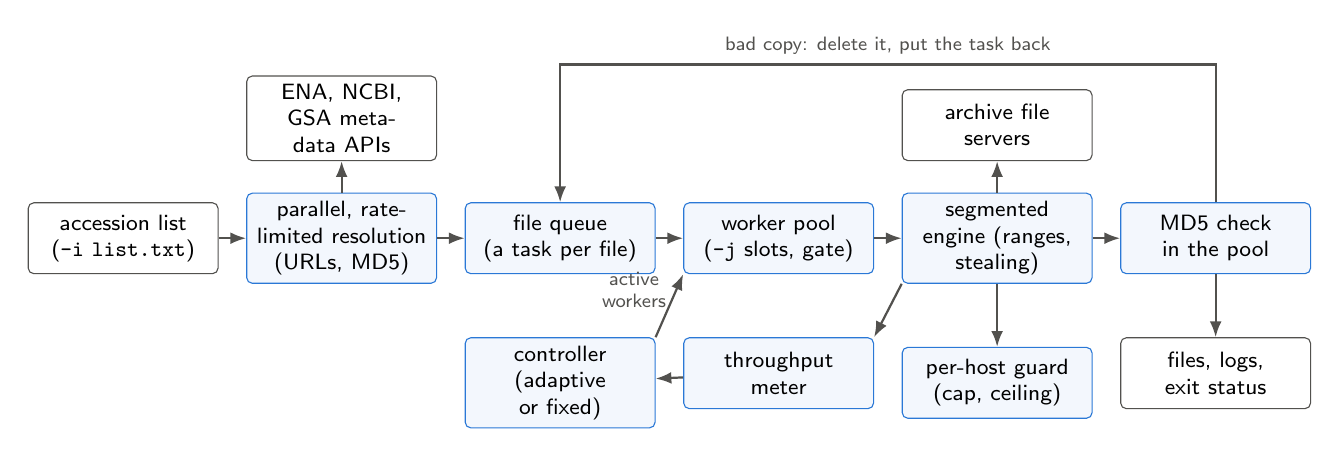
\begin{tikzpicture}[
  node distance=4mm and 3.5mm,
  box/.style={draw=aseq, fill=boxbg, rounded corners=2pt, align=center, font=\footnotesize, inner sep=3pt, minimum height=9mm, text width=2.2cm},
  ext/.style={draw=ink2, fill=white, rounded corners=2pt, align=center, font=\footnotesize, inner sep=3pt, minimum height=9mm, text width=2.2cm},
  arr/.style={-{Latex[length=2mm]}, draw=ink2, thick},
  lab/.style={font=\scriptsize, text=ink2, align=center}]
\node[ext] (list) {accession list\\(\texttt{-i list.txt})};
\node[box, right=of list] (res) {parallel, rate-limited resolution (URLs, MD5)};
\node[box, right=of res] (queue) {file queue\\(a task per file)};
\node[box, right=of queue] (pool) {worker pool\\(\texttt{-j} slots, gate)};
\node[box, right=of pool] (eng) {segmented engine (ranges, stealing)};
\node[box, right=of eng] (ver) {MD5 check in the pool};
\node[ext, above=of res] (api) {ENA, NCBI, GSA metadata APIs};
\node[ext, above=of eng] (arch) {archive file servers};
\node[box, below=8mm of queue] (ctrl) {controller (adaptive or fixed)};
\node[box, below=8mm of pool] (meter) {throughput meter};
\node[box, below=8mm of eng] (guard) {per-host guard (cap, ceiling)};
\node[ext, below=8mm of ver] (out) {files, logs, exit status};
\draw[arr] (list) -- (res); \draw[arr] (res) -- (api); \draw[arr] (res) -- (queue);
\draw[arr] (queue) -- (pool); \draw[arr] (pool) -- (eng); \draw[arr] (eng) -- (arch);
\draw[arr] (eng) -- (ver); \draw[arr] (ver) -- (out); \draw[arr] (eng) -- (guard);
\draw[arr] (eng.south west) -- (meter.north east); \draw[arr] (meter) -- (ctrl);
\draw[arr] (ctrl.north east) -- node[lab, left, pos=0.75]{active\\workers} (pool.south west);
\draw[arr] (ver.north) |- ++(0,1.75) -| node[lab, above, pos=0.25]{bad copy: delete it, put the task back} (queue.north);
\end{tikzpicture}
\end{document}
